\section{HLS based BFS optimization} \label{sec:bfs-opt}
As there are large amount of irregular memory accesses in BFS 
and they lead to rather low memory bandwidth 
utilization \cite{wang2017multikernel}, irregular memory access is a key 
factor that affects the BFS performance. Centering this problem, 
we propose a set of combined high-level optimizations including graph 
reordering, on-chip buffer partition 
and hyper BFS pipelining for efficient implementation 
with OpenCL on Intel Harp-v2. The optimizations are 
detailed in the rest of this section. 

%\subsection{Irregularity in BFS}
%\subsubsection{Irregular memory access}
%The basic BFS structure as mentioned in Figure \ref{fig:base-bfs} is well pipelined, 
%but it involves a large number of random memory accesses as analyzed 
%in \cite{Merrill2012scalable}. In the second stage, the vertex indices in the frontier 
%are usually not continuous, so the RPA read becomes random. For vertices with 
%larger degree, the CIA read can be considered as sequential memory access. Nevertheless, 
%the vertex degree of the graphs especially the social network follows the power-law 
%distribution and it indicates that there are a great number of low-degree vertices 
%and short sequential memory accesses. Particularly, since the vertex degree in 
%the BFS accelerator is known at run-time, the CIA read is usually aligned to the vertex 
%index data width (32 bits in this work). 
%
%In the third stage, when the status array 
%is located in the main memory, the status read is also random. When the vertex is un-visited, 
%random write is also required. In the last stage, frontier vertices typically write 
%sequentially because only part of the frontier neighbors become new frontiers 
%in the next BFS iteration, it is also random memory access by default. 
%While the frontier vertices are usually not sequential, the vertex level update 
%is also random. The massive random or short sequential
%memory accesses in combination result in the extremely low memory bandwidth utilization and 
%performance accordingly. 

%\subsubsection{Dependent data paths}

\subsection{Graph reordering}

To alleviate the irregular memory access in BFS, 
we propose a graph reordering scheme for the target accelerator. 
The basic idea is to optimize the edge layout for more efficient 
memory access or processing without changing the graph structure.
It needs to be done once for each graph and can be considered 
as graph pre-processing. Note that graph pre-processing covers 
many distinct methods such as graph partition and graph reordering. 
It is a common practice in many graph processing systems \cite{Dai2017foregraph}
\cite{ham2016graphicionado} \cite{gui2019survey} \cite{shi2018graph}.


As each frontier vertex may have multiple neighboring 
vertices or associated edges to be processed, sequential edge processing 
will soon become the bottleneck of the BFS. Parallel processing alleviates the bottleneck, 
but it is usually constrained by the memory access conflicts. Figure \ref{fig:write-conflict} 
shows the conflicts when inspecting the frontier neighbors in parallel.  
Both vertex 8 and Vertex 12 are neighbors of vertex 2 and they are supposed to be 
processed in parallel. However, the status or property of 
the two vertices may stay in the same DDR bank or on-chip buffer bank. As a result, 
they can only be written sequentially. The conflict is essentially caused by the 
limited memory level parallelism, so we call it memory conflict. 
There is also data dependency conflict. When the frontiers are processed in parallel, 
vertex 0 and 10 that have the same neighbor i.e. Vertex 3 and we can not perform status 
write of vertex 3 in parallel. We take it as data conflict. 
The data dependency remains despite the different data layouts, 
so we focus on resolving the memory conflict in this subsection.   

\begin{figure}
\center{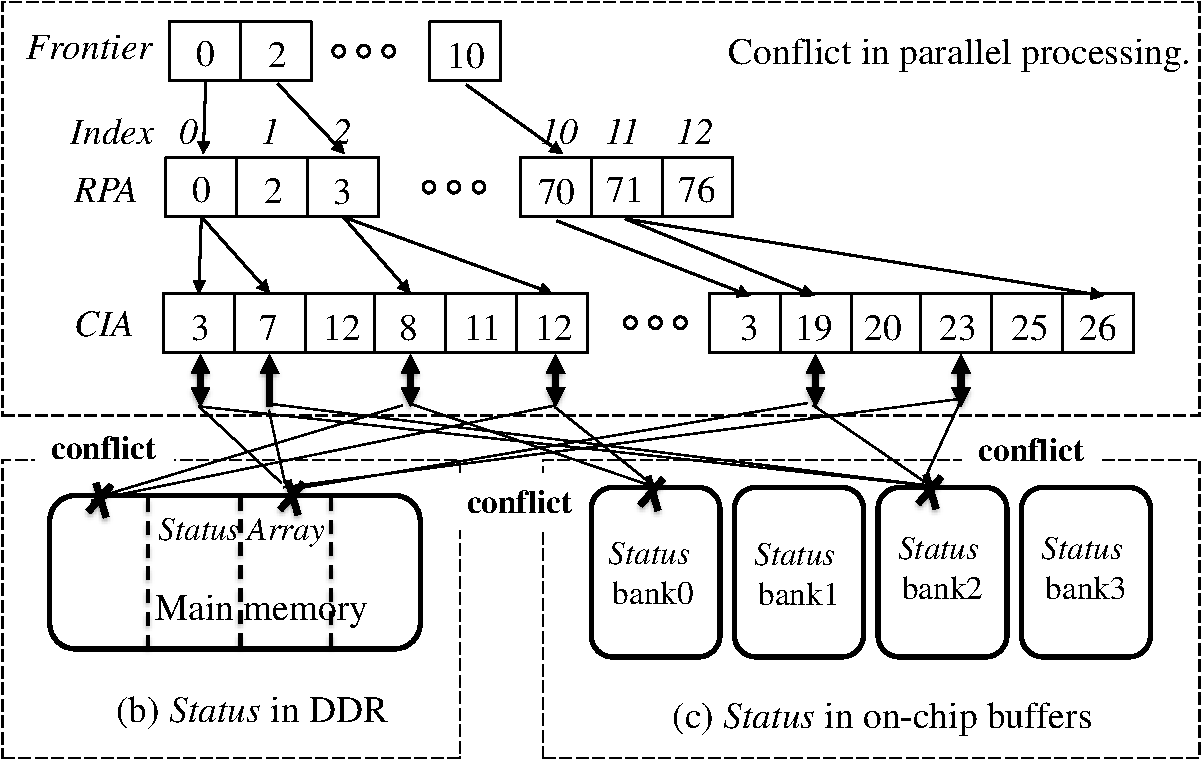
\includegraphics[width=0.7\linewidth]{write-conflict}}
    \caption{Conflicts among the parallel BFS data paths}
\label{fig:write-conflict}
\vspace{-0.5em}
\end{figure}

To address the memory conflict in BFS, we split the outgoing edges i.e. CIA array 
into batches and edges in each batch can be processed independently.
With the reordering and batching, the parallelization of the edge processing 
becomes straightforward and friendly to the high-level compilation tools.
Meanwhile, the batching enforces a coalesced CIA read and it is also beneficial to 
the efficiency of the memory accesses according to the experiments in Section \ref{sec:motivation}. 

This reordering can be performed offline. A typical example of the reordering is shown in Figure \ref{fig:graph-reorder}. 
The original CSR graph is placed in the top part of the figure. 
To divide the edges into batches for parallel processing, we reorder the edges i.e. CIA 
of each vertex. In this example, batch is set to be 2. For Vertex 0, 
it has as 2 neighbors i.e. Vertex 3 and 7 according to the RPA. 
We expect the vertices in each batch to be divided into distinct memory 
banks either in DDR banks or on-chip buffer banks so that there is no 
access conflict during processing. Here we just use the simple modular 
operation to divide the data, so Vertex 3 and 7 must be put into two batches.
The empty slot in each batch will be filled with -1 to notify the accelerator to 
ignore it during processing. Since the CIA is expanded after 
the reordering and batching, the RPA gets updated accordingly.
With the reordering and batching, more memory space is required to store the 
CSR graph. The advantage is the aligned memory access 
with higher data width and conflict-free edge processing, 
both of which are beneficial to the hardware implementation 
using Intel OpenCL.

\begin{figure}
\center{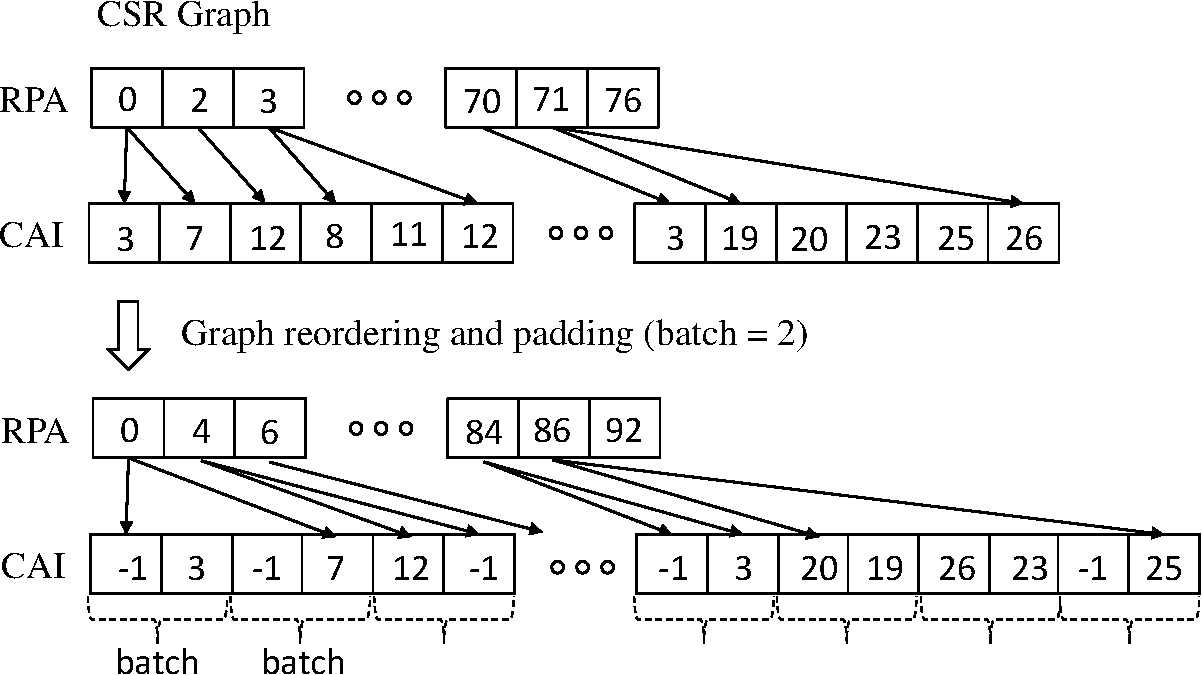
\includegraphics[width=0.72\linewidth]{graph-reorder}}
    \caption{CSR layout after the graph reordering and batching}
\label{fig:graph-reorder}
\vspace{-1em}
\end{figure}

\subsection{On-chip buffer partition}
To avoid frequent main memory access, we utilize bitmap to store 
the visiting status during BFS. Each vertex needs only one bit 
storage and the latest FPGAs with dozens of mega bits can accommodate 
graphs with dozens of millions of vertices such as twitter2010 graph which has 
around 42M vertices \cite{boldi2011layered}. In line with the graph reordering 
and batching, we split the visiting status bitmap into multiple banks that 
can be accessed in parallel. Suppose the batch size is $W$, we set the 
bitmap buffer partitions to be $W$ as well. The vertex visiting status will 
be evenly distributed across the bitmap buffer banks. The visiting status of 
vertex $id$ will be put into the $i$th memory bank where $i = mod(id, W)$.
As the vertex status read/write is mostly random and parallel in BFS, 
accessing the status via the on-chip buffer banks guarantees determined 
and low latency. It is much more efficient compared to the DDR 
accessing. 

Moreover, the parallel bitmap buffer banks further facilitate 
conflict-free processing as presented in Figure \ref{fig:bitmap}. 
In this example, $W = 8$ and it indicates that 8 edges can be 
processed in parallel. When a processing path gets -1 
from CIA stream, it will skip the rest of the processing as shown 
in the pseudo code in Figure \ref{fig:bitmap}.
Meanwhile, with the simplified and regular processing kernel, 
the initiation interval (II) of the kernel is 2 when implemented 
with Intel OpenCL. In contrast, the II of the crossbar based 
parallel processing kernels \cite{ham2016graphicionado} goes up to 6 
and it further requires the expensive crossbars and buffers. 
This is also a key factor that motivates us to adopt the reordering and 
batching approach despite the additional data padding.

\begin{figure}
\center{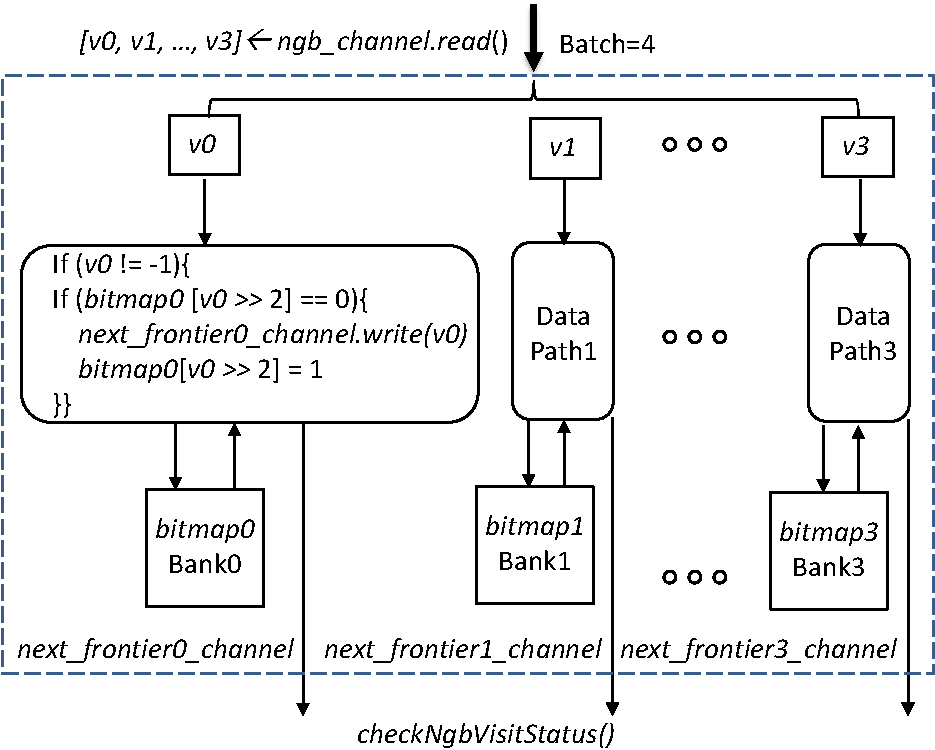
\includegraphics[width=0.67\linewidth]{bitmap}}
    \caption{Parallel visiting status bitmap buffer banks and conflict-free processing data paths}
\label{fig:bitmap}
\end{figure}

%\subsubsection{CPU assisted data reorganization}
%As discussed in Section \ref{sec:motivation}, irregular memory access with 
%small data width results in low memory bandwidth utilization. While the 
%attached host processor performs much better on random accesses because 
%of its memory hierarchy, we opt to offload these irregular memory accesses 
%to the host processor and reorganize the data for efficient FPGA processing. 
%Figure \ref{fig:reorg} shows the reorganization details. Instead 
%of going through the frontier reading and RPA reading sequentially for 
%frontier neighbors, we have the host processor to combine both processing steps 
%and gather the scattered RPA into a new slightly different RPA array.
%With the new RPA array, the accelerator can continue with sequential memory 
%accesses in the BFS iteration. This also ensures the whole pipeline stages of BFS to be 
%efficient. While the CPU based data reorganization needs to 
%transfer the data between CPU memory and FPGA host memory 
%when the CPU and FPGA have independent memory, the data transfer 
%may compensate the benefits. 
%
%We can also merge RPA of neighboring vertices such that 
%the amount of data in the new RPA array can be reduced. This 
%also helps to reduce the amount of memory read of CIA and thus 
%is beneficial to the resulting performance.
%The problem is whether we should sort the frontier vertices.
%Sorting takes quite some time but it brings more chances of 
%CIA access optimization.
%
%\begin{figure}
%	\center{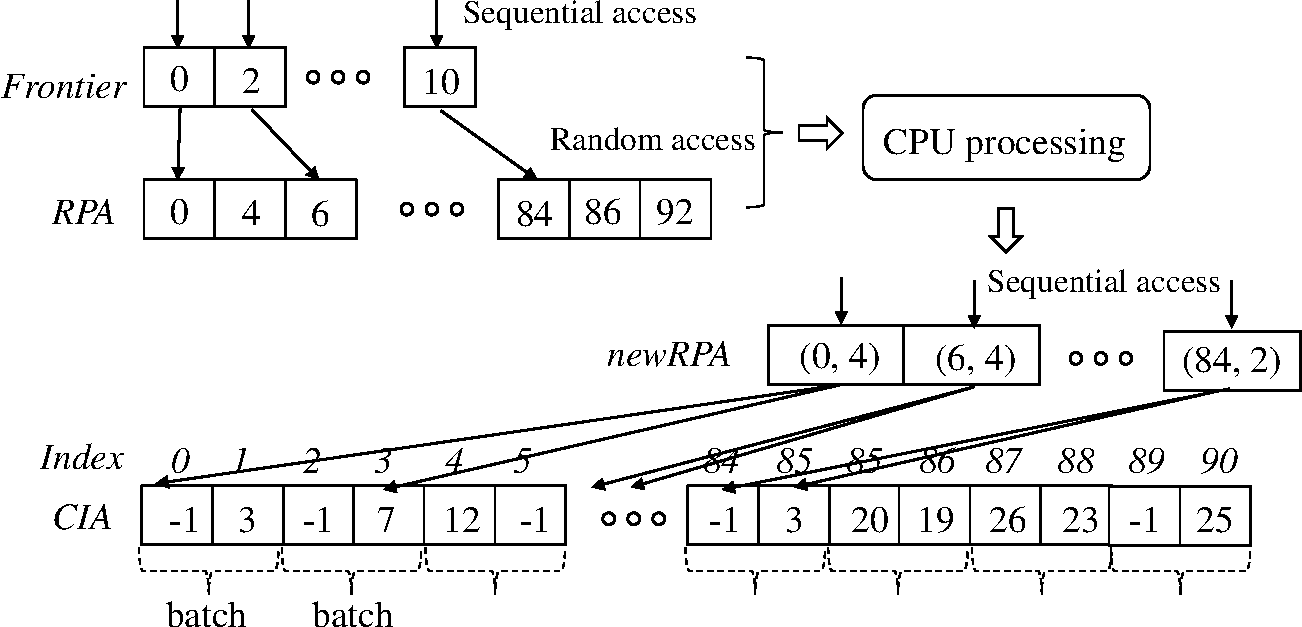
\includegraphics[width=0.85\linewidth]{reorg}}
%    \caption{RPA reorganization}
%\label{fig:reorg}
%\vspace{-1em}
%\end{figure}

\subsection{Hyper pipelining}
As mentioned in the above sub section, updating the level information of the active 
BFS frontier vertices are mostly random and time-consuming. While the classical BFS 
algorithm follows the bulk synchronous processing (BSP) model and the level update
affects each BFS iteration, BFS performance is influenced. We notice that the level update 
can actually be postponed as long as the frontier vertices are kept. With this observation, 
we propose a hyper pipelining approach as shown in Figure \ref{fig:hyper}. Basically, 
we separate the level update from the baseline BFS and overlap it within continuous BFS processing.  
As the level update is fast compared to the overall BFS, it can either be processed on CPU or FPGA 
with negligible influence on the main BFS processing. Currently, we just put it on host processor 
to ensure that the main BFS accelerator implementation frequency is not affected.
\begin{figure}
	\center{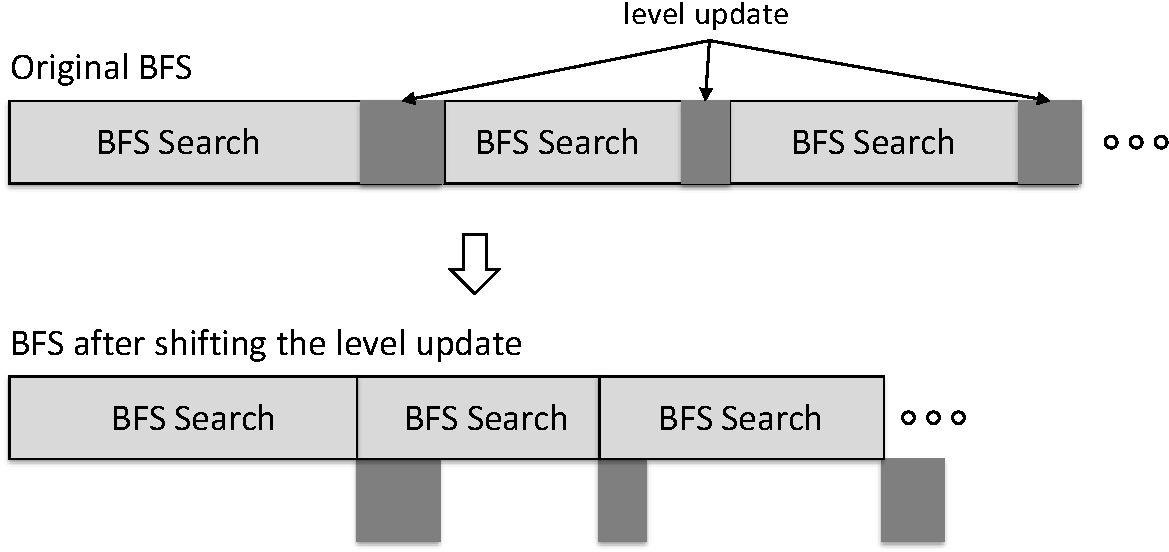
\includegraphics[width=0.7\linewidth]{hyper-pipeline}}
	\caption{Hyper pipelining}
\label{fig:hyper}
\vspace{-1em}
\end{figure}

\subsection{Optimized BFS structure}
With the above optimizations, the BFS structure is 
presented in Figure \ref{fig:opt-bfs}. The frontier inspection can be 
processed in parallel with the level update of previous BFS processing. 
The first two pipeline stages remain unchanged as they are not the 
performance bottleneck. In the third pipeline stage, 
random vertex status read and update over DDR is replaced with parallel 
on-chip buffer operations. In the last pipeline stage, level update is offloaded 
and hidden. Also we adopt the batch write to avoid random frontier vertices 
write to DDR. The irregular memory access in BFS is reduced dramatically.

\begin{figure}
	\center{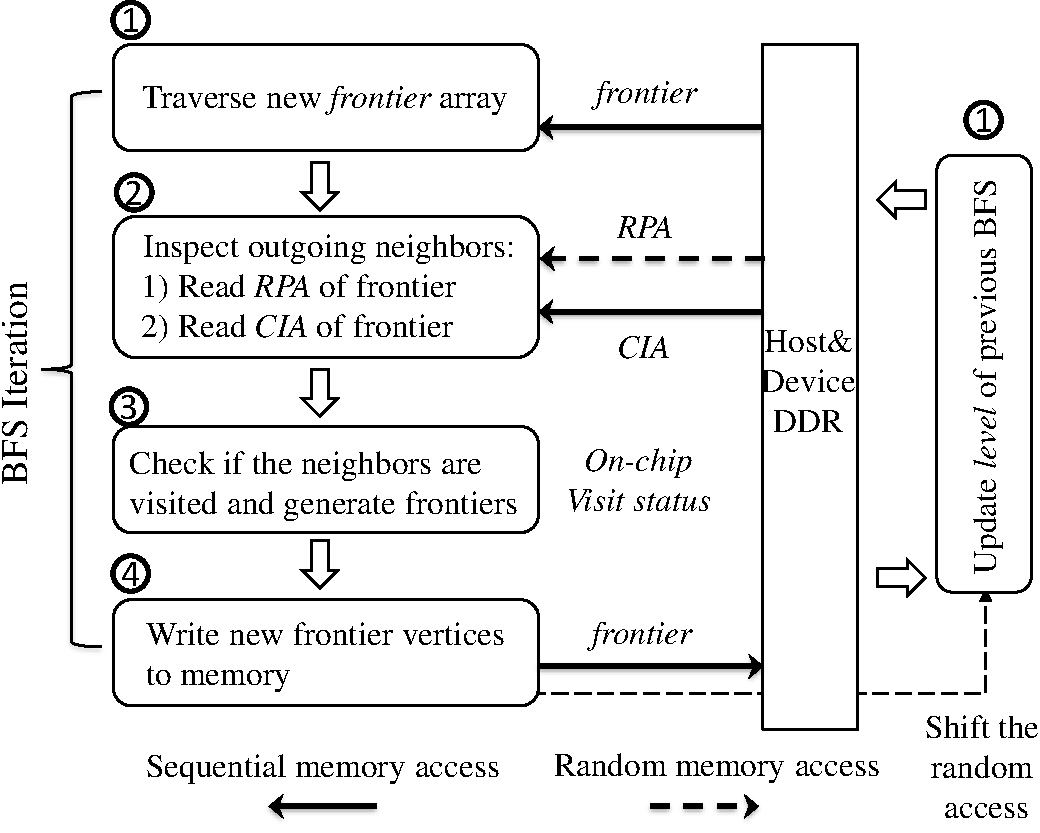
\includegraphics[width=0.75\linewidth]{opt-bfs}}
    \caption{Optimized BFS pipeline}
\label{fig:opt-bfs}
\vspace{-1em}
\end{figure}

